\section{Introdução}

Este documento foi realizado no âmbito da unidade
curricular de Análise de Dados, do curso de Engenharia
Informática do Instituto Superior de Engenharia do Porto.

O trabalho desenvolvido incidiu sobre um conjunto de dados de uma Operadora Móvel, mais concretamente sobre a situação anormal de perda de clientes.

Este mesmo trabalho teve como objetivo a Análise de Desempenho de Técnicas de Aprendizagem Automática e foram utilizados diversos algoritmos como: Regressão Linear, Árvores de Decisão, K-vizinhos-mais-próximos e Redes Neuronais. A ferramenta utilizada de forma a cumprir este objetivo foi R.

No próximo capítulo é apresentado o enquadramento teórico sobre os algoritmos utilizados no relatório. 

\subsection{Regressao Linear e Árvores de Regressão}

A regressão linear, bastante utilizada para se estimar um valor esperado de uma certa variável, tem por base num conjunto de variáveis: dependentes e independentes. As variáveis independentes (ou preditoras) são importantes para o calculo da variável que se deseja prever, sendo que cada uma tem a sua influencia naquilo que e o valor esperado/previsto. Resumidamente, a regressão linear tem 2 objetivos: analisar um conjunto de variáveis preditoras e a forma como estas mesmas impactam a variável dependente. A regressão linear pode ser caraterizada por dois tipos: regressão linear simples e regressão linear múltipla. 
[1]

A regressao linear simples traduz a previsão de uma variável com a introdução de apenas uma variável preditora, como traduz a formula seguinte: [2]

\begin{center}
{$$Yi = \beta_0 + \beta_1 \ast Xi + \xi_i$$}
\end{center}

A regressão linear múltipla traduz o cálculo da variável desejada introduzindo um conjunto de variáveis independentes:

\begin{center}
{$$Yi = \beta_0 + \beta_1 \ast X_1i + \beta_2 \ast X_2i + ... + \beta_k \ast \xi_i$$}
\end{center}

Ambos os modelos tem por objetivos determinar como duas ou mais variáveis se relacionam, estimar uma função que permita determinar a relação entre variáveis e usar essa equação resultante para prever valores possíveis para a variável dependente. Por um lado, regressão linear não determina qualquer relação causal, pode apenas dar pistas que podem ser testadas estatisticamente. [3]
Por outro lado, uma árvore de regressão é formada por nós de decisão e é uma ferramenta usada quando a variável dependente é quantitativa. A árvore de regressão é um exemplo de árvore de decisão e tem a função de calcular um valor médio de previsão para cada nó da árvore usando a soma de quadrados e analise de regressão. [4]

\subsection{Árvores de Decisão}

As Árvores de Decisão são uma ferramenta de suporte a decisões que mapeia todos os resultados possíveis a partir de uma série de escolhas. Estas consistem em um conjunto de nós de decisão, conectados por ramos, estendendo-se para baixo a partir do nó raiz até terminar em nós folha. Começando no nó raiz, que por convenção é colocado no topo do diagrama de árvore de decisão, as variáveis são testadas nos nós de decisão, com cada resultado possível resultando numa ramificação. Cada ramificação leva a outro nó de decisão ou a um nó folha final. As árvores também podem ser representadas por um conjunto de regras para melhorarem a legibilidade e a interpretabilidade humana. Estes métodos de aprendizagem estão entre os mais utilizados e têm sido aplicados a um grande número de campos (desde diagnóstico médico à gestão de risco de crédito na banca). 

Um dos exemplos mais conhecidos de uma árvore de decisão é o exemplo do ténis como observamos na Fig 1. Neste exemplo conseguimos determinar se é um ”bom dia para jogar ténis" através da Árvore de Decisão. Primeiro testa-se o nó de decisão "Outlook", gerando 3 ramos
possíveis, em que dois deles seguem para outro nó de decisão, e o outro vai diretamente para uma folha com a classificação, respondendo a pergunta inicial.
\begin{figure}[htbp]
\centerline{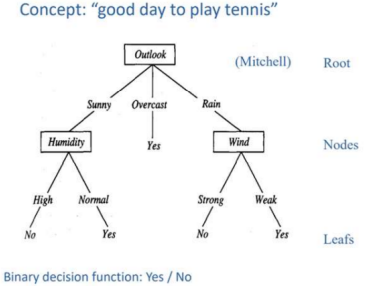
\includegraphics{images/tenis.png}}
\caption{Exemplo de uma arvore de decisão.}
\label{fig}
\end{figure}
[5]

Entre as vantagens das Árvores de Decisão, temos a facilidade com que são compreendidas ou capacidade de se decidir as melhores opções. A grande desvantagem presente é o facto de que estas se podem tornar excessivamente complexas, dificultando o processo de tomada de decisão. [6]

\subsection{Redes Neuronais}

Redes neuronais artificiais são o coração dos algoritmos de aprendizagem profunda, sendo elas inspiradas pela estrutura do cérebro humano e da comunicação biológica neuronal do mesmo. Estas têm um número surpreendente de características observadas no processo cognitivo do ser humano tal como aprendizagem pela experiência. Para construir um sistema destes, é necessário definir o número e tipo de neurónios e como estes se conectam entre si, colocar um peso entre eles e perceber quais destes pesos são apropriados para o problema em questão, o que se converte numa nova aprendizagem. [7]

As neural networks por norma consistem em três tipos de camadas: uma camada de input, uma ou mais camadas escondidas e uma camada de output, todas elas ligadas por
conexões com um determinado peso. A camada escondida é configurável pelo analista, quer em termos de número de camadas, mas também em quantidade de nós. Porém, A escolha da quantidade de nós pode por vezes ser complicada, porque apesar de uma grande quantidade de nós aumentar a flexibilidade e o poder da rede para identificar certos padrões, isto pode levar a overfitting o que afeta negativamente a
qualidade dos resultados. No entanto, caso sejam escolhidos poucos nós para a camada escondida, podemos ter um problema na precisão em treinos, indicando que é necessário ter mais nós. [7]

Um neurónio artificial acaba por ter como função a realização de uma operação a partir de determinados inputs e calcular e enviar o seu resultado. Isto é feito em duas fases: primeiramente calcula-se a soma dos pesos dos valores de entrada e de seguida calcula-se o valor de ativação do neurónio através de uma função de ativação ou de transferência. A soma dos pesos é calculada pelos pesos associados a determinados inputs e com o peso do offset como e visível na seguinte formula. [7]

\begin{center}
    {$$Xx1 \ast w1 + x2 \ast w2 + (\neg1) \ast \theta$$}
\end{center}

Posteriormente, a função de ativação irá verificar se o valor calculado no passo anterior é suficiente para ativar o neurónio, produzindo um output. Isto culmina num processo de aprendizagem através da backpropagation em que, na fase de treino, os valores do output são comparados com os valores reais calculando o valor do erro da previsão. De modo a minimizar os erros de previsão, a rede neuronal altera os pesos anteriores de acordo com o resultado obtido e volta a repetir o processo inicial. [7]
Redes neuronais podem ter vários tipos de topologias, todas elas com características diferentes: [7]
\begin{itemize}

\item \textbf{feed-forward networks} que são redes que apenas têm conexões numa direção, não havendo recursividade;    
\item \textbf{recurrent networks} caso tenham feedback loops;
\item \textbf{self-organized} caso não tenham um supervisor, tendo algoritmos de aprendizagem autónomos.

\end{itemize}
    
Estas estruturas podem ainda ser caracterizadas pelo seu número de camadas sendo que as monocamadas podem apenas resolver problemas de separação linear, quando as redes neuronais de multi-camadas, devido ao seu maior poder, conseguem resolver problemas mais complexos. [7]

\subsection{Cross-Validation}

Cross-validation é um método estatístico que é usado de modo a descobrir a eficiência de modelos de machine learning. Consiste em dividir os dados em conjuntos(partes), onde um conjunto é utilizado para treino e outro conjunto é utilizado para teste e avaliação do desempenho do modelo. A utilização do Cross-Validation tem altas chances de detetar se o modelo está em overfitting. [8]
Existem diversas técnicas para se fazer a cross-validation, havendo 4 em destaque:
[9]
\begin{itemize}
\item O metodo \textbf{Hold Out}, sendo o mais simples de todos em que se dividem os dados em 2 partes, sendo uma parte de treino e outra de teste. O nosso modelo é treinado com a parte de treino e posteriormente é pedido para prever os dados de teste. De seguida são comparados os resultados da previsão, com os dados verdadeiros.

\item O metodo \textbf{K-fold cross-validation} que é um método modificado do método holdout, em que os dados são divididos em K subsets, em que K é um valor idealmente compreendido entre 5 e 10, sendo que quanto menor o K, mais semelhantes irão ser os resultados comparativamente ao método hold out. De seguida, treinamos o modelo usando k-1 ”folds”, validando e testando o modelo no K fold restante. Este processo é repetido até que cada K-fold seja usado como teste no modelo.

\item O metodo \textbf{Repeated K-Fold cross-validation} que consiste em aplicar o método anterior, K-Fold cross-validation mais do que uma vez

\item O método \textbf{Leave one out cross-validation} em que se maximiza o K-Fold cross-validation, igualando o K ao (N) número de entradas nos nossos dados. Este método é aplicado N vezes, onde se treina o modelo com todos os dados exceto 1, sendo feita uma previsão para o mesmo e testando o modelo. O erro de previsão irá ser a média de todas as estimativas de erro obtidas anteriormente.
\end{itemize}

Os modelos de regressão também têm a sua performance medida, sendo isto feito através da determinação da precisão do modelo na previsão de dados que não são usados na construção do modelo. Algumas das métricas usadas para quantificar a performance dos modelos de regressão são: [9]
\begin{itemize}
\item \textbf{R-squared} que representa a correlação quadrada entre os valores previstos e os obtidos, em que quanto maior o R2, melhor o modelo. Regra geral, este é o critério usado em regressão linear.

\item \textbf{Root Mean Squared Error} que mede o valor médio do erro de previsão do modelo na previsão dos valores, ou seja, a diferença média entre os valores previstos e os valores obtidos. Quanto menor o RMSE, melhor é a performance do modelo.

\item \textbf{Mean Absolute Error} que é uma alternativa ao Root Mean Squared Error que apresenta a diferença de ser menos sensível a outliers. Corresponde à diferença média absoluta entre os valores previstos e os obtidos, e quanto menor o MAE, melhor a performance do modelo.
\end{itemize}

\subsection{K-vizinhos-mais-próximos}
No ramo da inteligência artificial, alguns dos métodos de classificação mais usados é o dos Nearest Neighbours (NN) e o dos K-vizinhos-mais-próximos (KNN). Estes algoritmos têm como objetivo classificar os dados de uma dada instância com base nos seus vizinhos mais próximos sendo que o algoritmo dos vizinhos mais próximos o faz para K = 1, enquanto que o KNN o faz para os K vizinhos mais próximos. Estes algoritmos são dos mais simples de supervisionar e são dos mais estudados na inteligência artificial. [10]

Os algoritmos de K vizinhos mais próximos acabam por ser algoritmos de aprendizagem preguiçosa, pois estes guardam os dados de exemplo de treino deixando o processamento dos mesmos em ”pausa” até a criação de novas previsões. De modo a fazer uma previsão, o KNN encontra os K vizinhos mais próximos de um determinado ponto e calcula a sua classificação ou a sua regressão com base nos vizinhos. Para executar estes algoritmos é necessário determinar o K, o que por vezes pode não ser fácil, pois caso o seu valor seja demasiado baixo, os resultados podem ser sensíveis a ”barulho” levando a resultados mais instáveis. Pelo outro lado, valores altos de K podem levar a que os vizinhos mais próximos incluam pontos de outras classes ou que a carga computacional aumente. [10]
Os algoritmos de vizinhos mais próximos para além de serem preguiçosos, podem ser postos noutras categorias, sendo também não paramétricos e discriminativos. [10]
Estes algoritmos são bastante importantes sendo usados em diversas áreas, nomeadamente na interseção entre a classificação de padrões, a visão computacional, reconhecimento de imagem e vídeos e a biometria e em sistemas de recomendação. [10]
